% https://shantoroy.com/latex/draw-multiple-y-axis-in-latex-pgfplot/
\documentclass{standalone}
\usepackage{pgfplots, pgfplotstable}

\begin{document}
    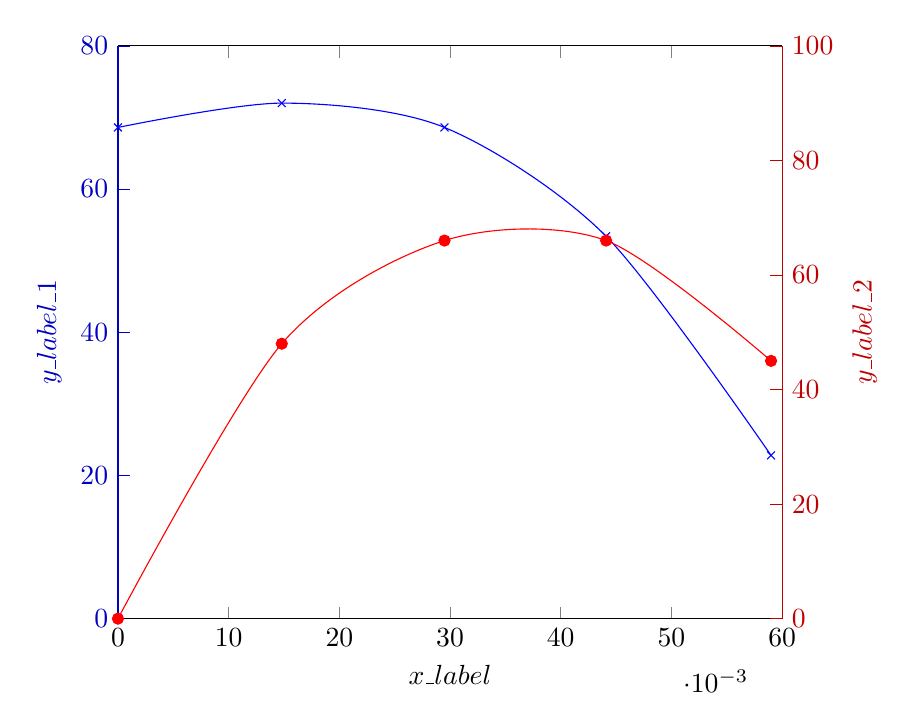
\begin{tikzpicture}
    \pgfplotsset{
        scale only axis,
        scaled x ticks=base 10:3,
        xmin=0, xmax=0.06,
        y axis style/.style={
            yticklabel style=#1,
            ylabel style=#1,
            y axis line style=#1,
            ytick style=#1
       }
    }
    
    \begin{axis}[
      axis y line*=left,
      y axis style=blue!75!black,
      ymin=0, ymax=80,
      xlabel=$x\_label$,
      ylabel=$y\_label\_1$
    ]
    \addplot[smooth,mark=x,blue] 
      coordinates{
        (0,68.6)
        (0.0148,72) 
        (0.0295,68.6)
        (0.0441,53.4)
        (0.059,22.8) 
    };
    \end{axis}
    
    \begin{axis}[
      axis y line*=right,
      axis x line=none,
      ymin=0, ymax=100,
      ylabel=$y\_label\_2$,
      y axis style=red!75!black
    ]
    \addplot[smooth,mark=*,red] 
      coordinates{
        (0,0)
        (0.0148,48) 
        (0.0295,66)
        (0.0441,66)
        (0.059,45.0) 
    };
    \end{axis}    
    \end{tikzpicture}

\end{document}
